\documentclass[pdftex,letterpaper,12pt]{report}
\usepackage{thesis}
\usepackage{amsmath}
\usepackage{amssymb}
\usepackage{amsthm}
\usepackage{mathtools}
\usepackage{bm}
\usepackage{gensymb}
\usepackage{wasysym}
\usepackage{mathtools}
\usepackage{physics}
\usepackage{empheq}
\usepackage{cases}
\usepackage{rotating}
\usepackage{subfig}
\usepackage{caption}
\usepackage{multirow}
\captionsetup{labelfont=bf} 
\captionsetup[subfloat]{position=top,singlelinecheck=off,justification=raggedright,font=bf,labelfont=large,labelformat=simple,captionskip=-2mm}
\usepackage{float}
\usepackage{enumitem} 
\usepackage[toc,page]{appendix}






\begin{document}
	
\begin{subequations}\label{InitialSpinup}
	\begin{gather}
	P_{pc}(t)=\gamma_{se}P_{A}t-\frac{1}{2}\gamma_{se}P_{A}(\gamma_{se}+\Gamma_{pc}+d_{pc})t^{2}\\
	P_{tc}(t)=\frac{1}{2}\gamma_{se}P_{A}d_{tc}t^{2}
	\end{gather}
\end{subequations}

This is a test:
\begin{equation}
\frac{1}{T}=\frac{1}{T_K}\frac{S}{V}\int_{0}^{\infty} f\left(l\right)^2 e^{-U\left(l\right)/kT}dl
\end{equation}
$Al(NO_3)_39H_2O$

\begin{table*}\scriptsize
	\captionsetup{font=scriptsize}
	\begin{center}
		\def\arraystretch{0.75}
		\setlength\tabcolsep{1pt}
		\begin{tabular}{|c|c|cccc|c|}
			\hline
			Cell & T($^\circ$C) & $X_1$ & $X_2$ & $X_3$ & $X_4$ & $X_{12}/X_{1234}$\\ 
			\multirow{2}{*}{Simone} & 215 & -0.02(12) & -0.10(14) & - & - & -0.04(12) \\
			& 255 & 0.13(08) & 0.08(09) & - & - & 0.11(06) \\
			\hline
			\multirow{4}{*}{Sosa} & 160 & 0.22(07) & 0.28(09) & 0.32(15) & 0.18(09) & 0.24(06)$^\dagger$ \\
			& 170 & 0.24(07) & 0.37(15) & - & - & 0.27(06)\\
			& 180 & 0.45(08) & 0.40(09) & 0.50(17) & 0.45(09) & 0.43(06)$^\dagger$ \\
			& 190 & 0.59(16) & 0.57(17) & - & - & 0.58(12) \\
			\hline
			\hline
			Boris & 235 & 0.21(14) & 0.31(14) & - & - & 0.26(10)\\
			\hline
			Sam. & 235 & 0.08(06) & 0.22(09) & - & - & 0.12(05) \\
			\hline
			Alex & 235 & 0.34(09) & 0.35(09) & 0.63(20) & 0.29(10) & 0.34(06)$^\dagger$\\
			\hline
			Astral & 235 & 0.15(07) & 0.22(10) & 0.20(14) & 0.14(07) & 0.17(05)$^\dagger$\\
			\hline
			Steph. & 235 & 0.31(17) & 0.31(10) & - & - & 0.31(08)\\
			\hline
			Brady & 235 & 0.13(07) & 0.15(09) & 0.23(14) & 0.11(07) & 0.14(05)$^\dagger$\\
			\hline
			\multirow{3}{*}{Antoinette} & 215 & 0.27(09) & 0.44(17) & 0.30(19) & 0.25(11) & 0.28(08)$^\dagger$\\
			& 235 & 0.20(09) & 0.34(12) & 0.36(17) & 0.15(09) & 0.24(07)$^\dagger$\\
			& 255 & 0.55(26) & 0.54(16) & 0.50(30) & 0.56(26) & 0.55(13)$^\dagger$\\
			\hline
		\end{tabular}
		\caption
		{Shown are the values of the X factor at the indicated over set temperatures. The last column is a weighted average of results from either the first two methods or all four methods. A $^\dagger$ indicates combined values computed with all 4 methods.}
		\label{table:Xtable}
	\end{center}
\end{table*}

\begin{figure}[H]
	\centering
	\resizebox{0.91\textwidth}{!}{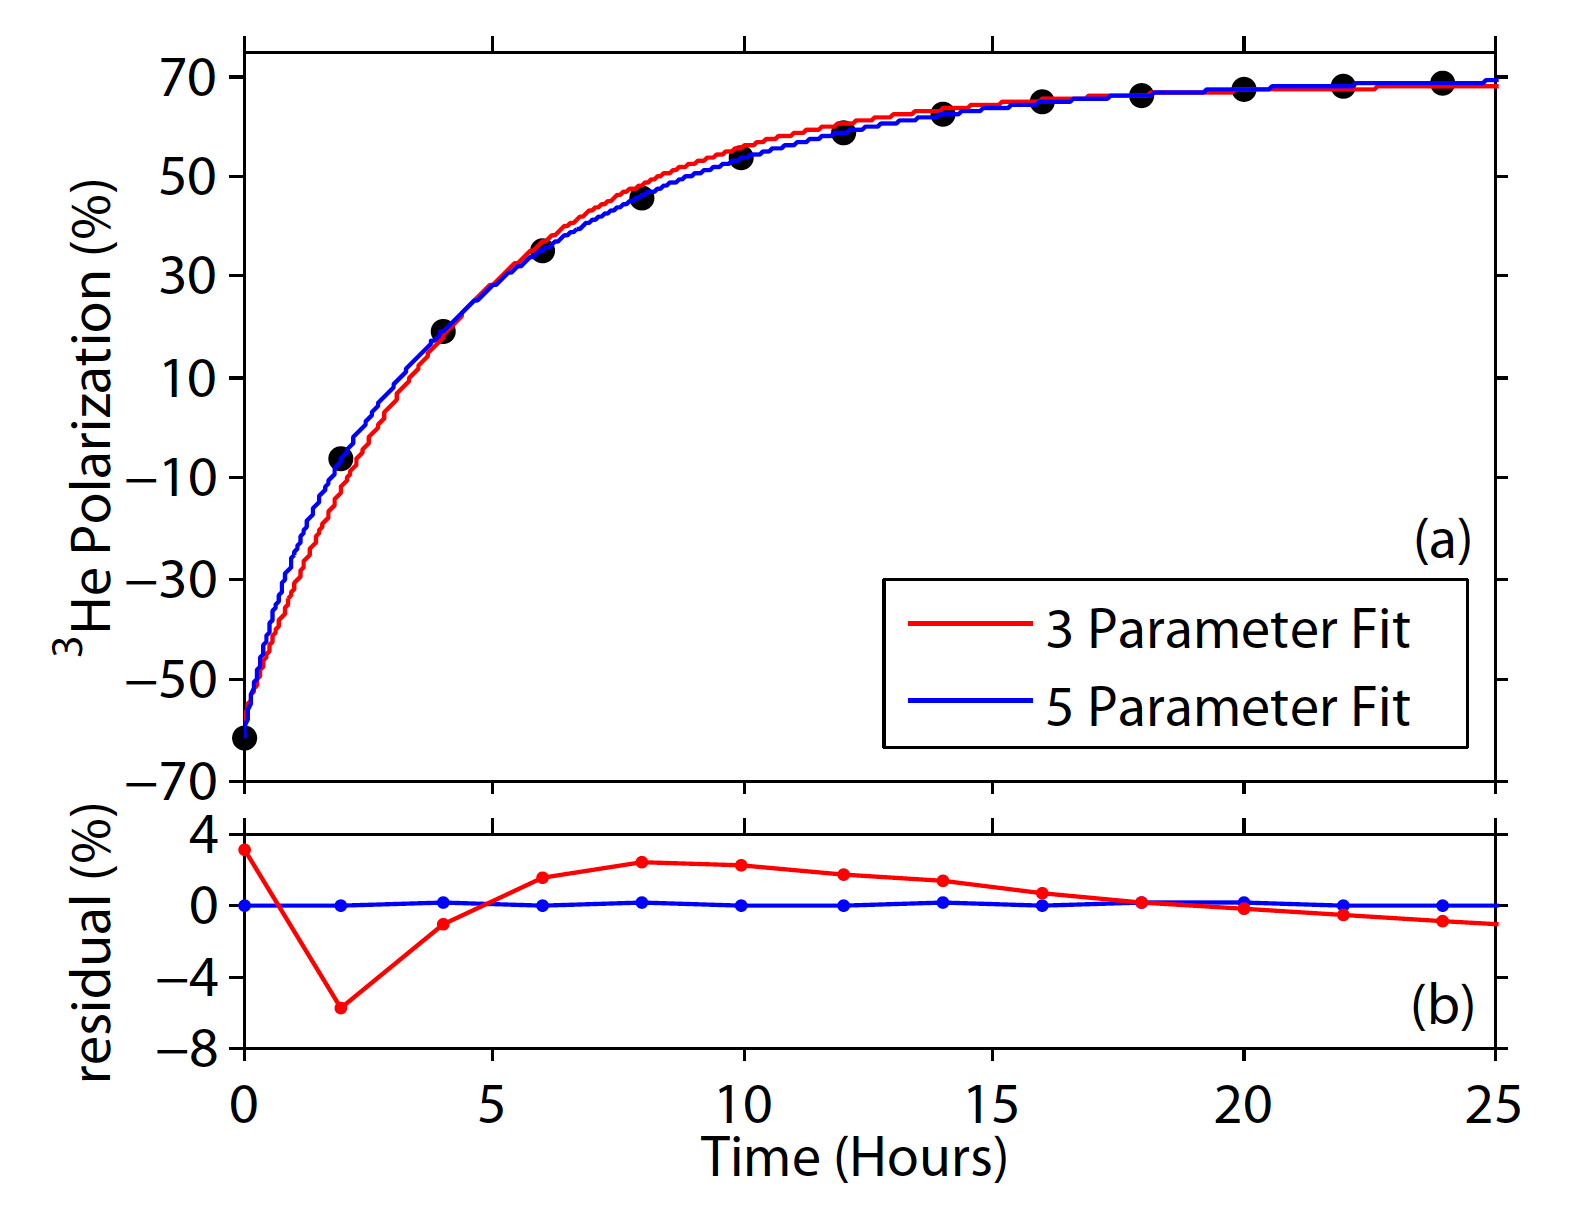
\includegraphics{Spinup.png}}
	\caption{{(a) Shown is a spinup of the target Brady. The spinup data has been fit with a 3-parameter and a 5-parameter formalism. (b) The residuals of the two fits. The error for 3-parameter fit is larger because it does not account for diffusion between two chambers. Adopted from~\cite{PhysRevC.91.055205}.}}
	\label{spinup}
\end{figure}

See in Fig.~\ref{spinup}


	
The energy levels of $^{87}$Rb are shown in Fig.~\ref{fig:foms}.
where $\Gamma_{A}$ is the pressure dependent FWHM, $\Gamma_{A}\approx 0.04nm/amg \cdot [^{3}He]$.

\addcontentsline{toc}{chapter}{Bibliography}
\bibliography{ref}

\end{document}